% Study-design figure, drawn in TikZ so the maths is typeset rather than
% approximated and the output is vector at any scale.
%
% Build:  python paper/make_design_figure.py
% which writes fig_design_data.tex (the cohort sizes, read from the result
% files so the figure cannot advertise data the repository does not contain)
% and then compiles this file to results/figures/fig_design.pdf.
\documentclass[border=5pt,multi,tikz]{standalone}
\usepackage[T1]{fontenc}
\usepackage{lmodern}
\usepackage{amsmath,amssymb}
\usepackage{xcolor}
\usetikzlibrary{arrows.meta,positioning,fit,backgrounds,calc}

\IfFileExists{fig_design_data.tex}{%% AUTO-GENERATED by paper/make_design_figure.py: DO NOT EDIT.
\newcommand{\NPhys}{30}
\newcommand{\NBci}{9}
\newcommand{\NCho}{52}
}{%
  \newcommand{\NPhys}{104}\newcommand{\NBci}{9}\newcommand{\NCho}{52}}

% No hyphenation anywhere: a diagram that breaks "density ma-trix" across a
% line reads as carelessness before anyone gets to the content.
\hyphenpenalty=10000 \exhyphenpenalty=10000 \tolerance=9999
\newcommand{\midsp}{\;}

% Palette: soft fills with a darker stroke of the same hue, which keeps a
% dense diagram legible in print and in greyscale.
\definecolor{cData}{HTML}{2A78D6}
\definecolor{cSensor}{HTML}{EB6834}
\definecolor{cRef}{HTML}{1BAF7A}
\definecolor{cClass}{HTML}{2A78D6}
\definecolor{cTwin}{HTML}{1BAF7A}
\definecolor{cQuant}{HTML}{EB6834}
\definecolor{cCirc}{HTML}{E87BA4}
\definecolor{cEval}{HTML}{7B61C4}
\definecolor{cInk}{HTML}{1A1A1A}
\definecolor{cMuted}{HTML}{6B6A66}

\begin{document}
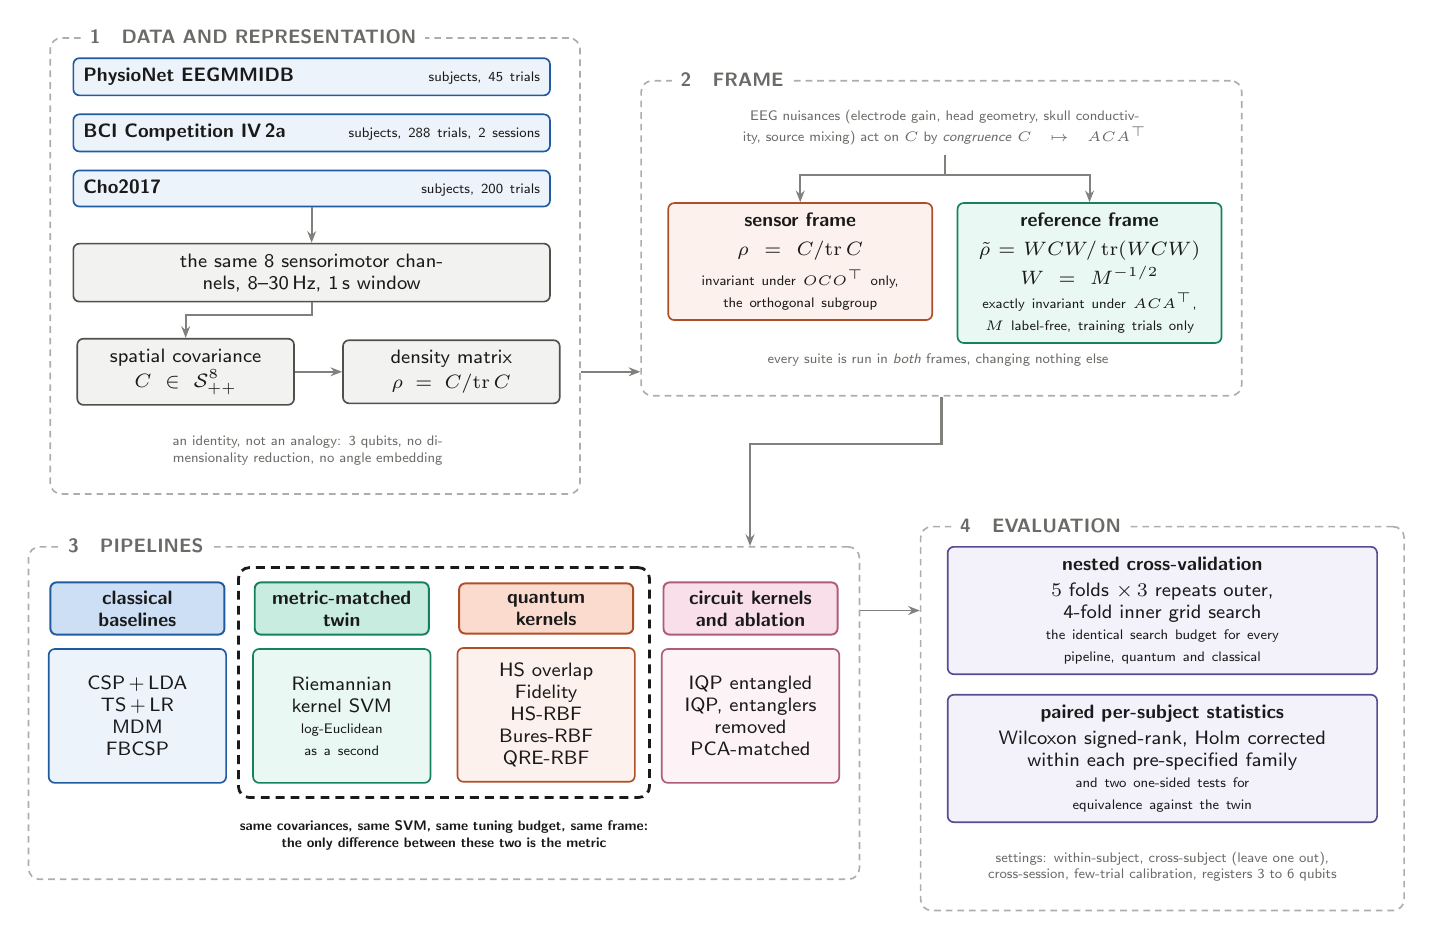
\begin{tikzpicture}[
  font=\sffamily\scriptsize,
  >={Stealth[length=4.2pt,width=3.2pt]},
  blk/.style={
    rounded corners=2.2pt, draw=#1!75!black, fill=#1!9, line width=0.6pt,
    align=center, inner sep=3.6pt, text=cInk},
  hdr/.style={
    rounded corners=2.2pt, draw=#1!75!black, fill=#1!24, line width=0.7pt,
    align=center, inner sep=3pt, font=\sffamily\scriptsize\bfseries, text=cInk},
  grp/.style={
    rounded corners=4pt, draw=cMuted!55, line width=0.6pt,
    dash pattern=on 2.4pt off 1.8pt, inner sep=7pt},
  ctrl/.style={
    rounded corners=4pt, draw=cInk, line width=1.0pt,
    dash pattern=on 3.2pt off 2.2pt, inner sep=5pt},
  tag/.style={
    font=\sffamily\scriptsize\bfseries, text=cMuted, fill=white, inner xsep=3pt,
    inner ysep=1pt},
  note/.style={font=\sffamily\tiny, text=cMuted, align=center},
  ar/.style={->, draw=cMuted!85, line width=0.7pt},
]

%% ============================================================== 1. DATA
\node[blk=cData, text width=58mm] (d1)
  {\textbf{PhysioNet EEGMMIDB}\hfill\tiny \NPhys{} subjects, 45 trials};
\node[blk=cData, text width=58mm, below=2.2mm of d1] (d2)
  {\textbf{BCI Competition IV\,2a}\hfill\tiny \NBci{} subjects, 288 trials, 2 sessions};
\node[blk=cData, text width=58mm, below=2.2mm of d2] (d3)
  {\textbf{Cho2017}\hfill\tiny \NCho{} subjects, 200 trials};

\node[blk=cMuted, text width=58mm, below=4.5mm of d3] (prep)
  {the same 8 sensorimotor channels, 8--30\,Hz, 1\,s window};

\node[blk=cMuted, text width=25mm, below=4.5mm of prep.south, anchor=north,
      xshift=-16mm] (cov)
  {spatial covariance\\[1pt]$C\in\mathcal{S}^{8}_{++}$};
\node[blk=cMuted, text width=25mm, right=6mm of cov] (rho)
  {density matrix\\[1pt]$\rho=C/\mathrm{tr}\,C$};
\draw[ar] (cov) -- (rho);

\node[note, below=2.6mm of cov.south, anchor=north, xshift=15.5mm,
      text width=58mm] (idnote)
  {an identity, not an analogy: 3 qubits, no dimensionality reduction,
   no angle embedding};

\draw[ar] (d3.south) -- (prep.north);
\draw[ar] (prep.south) -- ++(0,-1.6mm) -| (cov.north);

\begin{scope}[on background layer]
  \node[grp, fit=(d1)(d3)(prep)(cov)(rho)(idnote)] (gData) {};
\end{scope}
\node[tag, anchor=west] at ([xshift=4mm]gData.north west) {1\quad DATA AND REPRESENTATION};

%% ============================================================= 2. FRAME
\node[note, right=11mm of gData.north east, anchor=north west,
      text width=68mm, yshift=-8mm] (nuis)
  {EEG nuisances (electrode gain, head geometry, skull conductivity,
   source mixing) act on $C$ by \emph{congruence} $C\mapsto ACA^{\top}$};

\node[blk=cSensor, text width=31mm, below=6mm of nuis.south west, anchor=north west]
  (sensor)
  {\textbf{sensor frame}\\[2.5pt]
   $\rho=C/\mathrm{tr}\,C$\\[2.5pt]
   \tiny invariant under $OCO^{\top}$ only,\\\tiny the orthogonal subgroup};
\node[blk=cRef, text width=31mm, below=6mm of nuis.south east, anchor=north east]
  (ref)
  {\textbf{reference frame}\\[2.5pt]
   $\tilde\rho=WCW/\operatorname{tr}(WCW)$\\[1pt]
   $W=M^{-1/2}$\\[2.5pt]
   \tiny exactly invariant under $ACA^{\top}$,\\\tiny $M$ label-free, training trials only};

\coordinate (fmid) at ($(nuis.south)+(0,-2.6mm)$);
\draw[ar] (nuis.south) -- (fmid) -| (sensor.north);
\draw[ar] (nuis.south) -- (fmid) -| (ref.north);

\node[note, below=3mm of sensor.south, anchor=north, xshift=17.5mm,
      text width=68mm] (bothfr)
  {every suite is run in \emph{both} frames, changing nothing else};

\begin{scope}[on background layer]
  \node[grp, fit=(nuis)(sensor)(ref)(bothfr)] (gFrame) {};
\end{scope}
\node[tag, anchor=west] at ([xshift=4mm]gFrame.north west) {2\quad FRAME};

\draw[ar] (gData.east |- rho) -- (gFrame.west |- rho);

%% ========================================================= 3. PIPELINES
\node[hdr=cClass, text width=20mm, minimum height=6.2mm, below=11mm of gData.south west, anchor=north west]
  (h1) {classical\\baselines};
\node[blk=cClass, text width=20mm, minimum height=17mm, below=1.6mm of h1] (p1)
  {CSP\,+\,LDA\\ TS\,+\,LR\\ MDM\\ FBCSP};

\node[hdr=cTwin, text width=20mm, minimum height=6.2mm, right=3.6mm of h1] (h2) {metric-matched\\twin};
\node[blk=cTwin, text width=20mm, minimum height=17mm, below=1.6mm of h2] (p2)
  {Riemannian\\ kernel SVM\\[1.5pt]\tiny log-Euclidean\\\tiny as a second};

\node[hdr=cQuant, text width=20mm, minimum height=6.2mm, right=3.6mm of h2] (h3) {quantum\\kernels};
\node[blk=cQuant, text width=20mm, minimum height=17mm, below=1.6mm of h3] (p3)
  {HS overlap\\ Fidelity\\ HS-RBF\\ Bures-RBF\\ QRE-RBF};

\node[hdr=cCirc, text width=20mm, minimum height=6.2mm, right=3.6mm of h3] (h4) {circuit kernels\\and ablation};
\node[blk=cCirc, text width=20mm, minimum height=17mm, below=1.6mm of h4] (p4)
  {IQP entangled\\ IQP, entanglers\\ removed\\ PCA-matched};

\begin{scope}[on background layer]
  \node[ctrl, fit=(h2)(p2)(h3)(p3)] (gCtrl) {};
\end{scope}
\node[below=1.6mm of gCtrl.south, anchor=north, text width=54mm, align=center,
      font=\sffamily\tiny, text=cInk] (ctrlnote)
  {\textbf{same covariances, same SVM, same tuning budget, same frame:}\\
   \textbf{the \emph{only} difference between these two is the metric}};

\begin{scope}[on background layer]
  \node[grp, fit=(h1)(p1)(h4)(p4)(gCtrl)(ctrlnote)] (gPipe) {};
\end{scope}
\node[tag, anchor=west] at ([xshift=4mm]gPipe.north west) {3\quad PIPELINES};

% Down the right, so it never crosses the data panel or its caption.
\draw[ar, line width=0.9pt] (gFrame.south) -- ++(0,-6mm) -| ([xshift=-14mm]gPipe.north east);

%% ======================================================== 4. EVALUATION
\node[blk=cEval, text width=52mm, right=11mm of gPipe.north east, anchor=north west]
  (cv)
  {\textbf{nested cross-validation}\\[1.5pt]
   $5$ folds $\times\,3$ repeats outer,\\ 4-fold inner grid search\\[1.5pt]
   \tiny the identical search budget for every\\\tiny pipeline, quantum and classical};
\node[blk=cEval, text width=52mm, below=2.4mm of cv] (stat)
  {\textbf{paired per-subject statistics}\\[1.5pt]
   Wilcoxon signed-rank, Holm corrected\\ within each pre-specified family\\[1.5pt]
   \tiny and two one-sided tests for\\\tiny equivalence against the twin};
\node[note, below=2.4mm of stat, text width=54mm] (settings)
  {settings: within-subject, cross-subject (leave one out), cross-session,
   few-trial calibration, registers 3 to 6 qubits};

\begin{scope}[on background layer]
  \node[grp, fit=(cv)(stat)(settings)] (gEval) {};
\end{scope}
\node[tag, anchor=west] at ([xshift=4mm]gEval.north west) {4\quad EVALUATION};

\draw[ar] (gPipe.east |- cv) -- (gEval.west |- cv);

\end{tikzpicture}
\end{document}
